\documentclass{article}
\usepackage{tikz}
\usetikzlibrary{arrows.meta}

\begin{document}

\begin{figure}[h]
    \centering
    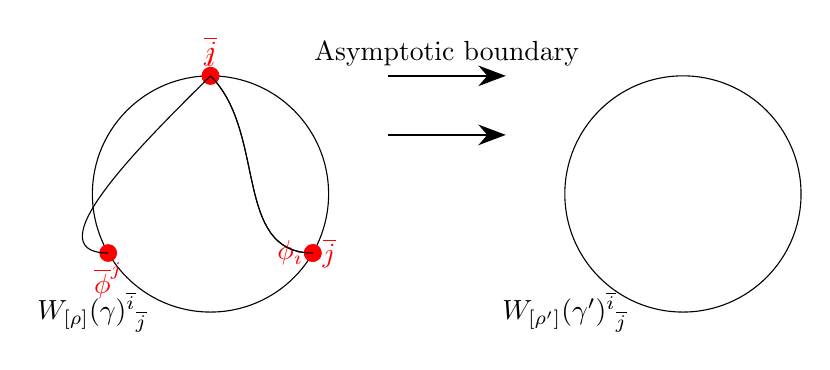
\begin{tikzpicture}[scale=1.5]

        % Circle (a)
        \draw (0,0) circle (1);
        \filldraw[red] (90:1) circle (2pt) node[above] {$i$};
        \filldraw[red] (-30:1) circle (2pt) node[right] {$\overline{j}$};
        \draw (90:1) to[out=-45,in=180] (-30:1);
        \node at (-1,-1) {$W_{[\rho]}(\gamma)^{\overline{i}}{}_{\overline{j}}$};

        % Circle (b)
        \draw (4,0) circle (1);
        \filldraw[red] (90:1) circle (2pt) node[above] {$\overline{j}$};
        \filldraw[red] (-30:1) circle (2pt) node[left] {$\phi_i$};
        \filldraw[red] (210:1) circle (2pt) node[below] {$\overline{\phi}^j$};
        \draw (90:1) to[out=-45,in=180] (-30:1);
        \draw (90:1) to[out=-135,in=180] (210:1);
        \node at (3,-1) {$W_{[\rho']}(\gamma')^{\overline{i}}{}_{\overline{j}}$};

        % Arrows
        \draw[-{Stealth[scale=1.5]},thick] (1.5,1) -- (2.5,1) node[midway,above] {Asymptotic boundary};
        \draw[-{Stealth[scale=1.5]},thick] (1.5,0.5) -- (2.5,0.5);

    \end{tikzpicture}
    \caption{(a) and (b)}
\end{figure}

\end{document}